\documentclass[11pt,a4paper,]{article}
\usepackage{lmodern}

\usepackage{amssymb,amsmath}
\usepackage{ifxetex,ifluatex}
\usepackage{fixltx2e} % provides \textsubscript
\ifnum 0\ifxetex 1\fi\ifluatex 1\fi=0 % if pdftex
  \usepackage[T1]{fontenc}
  \usepackage[utf8]{inputenc}
\else % if luatex or xelatex
  \usepackage{unicode-math}
  \defaultfontfeatures{Ligatures=TeX,Scale=MatchLowercase}
\fi
% use upquote if available, for straight quotes in verbatim environments
\IfFileExists{upquote.sty}{\usepackage{upquote}}{}
% use microtype if available
\IfFileExists{microtype.sty}{%
\usepackage[]{microtype}
\UseMicrotypeSet[protrusion]{basicmath} % disable protrusion for tt fonts
}{}
\PassOptionsToPackage{hyphens}{url} % url is loaded by hyperref
\usepackage[unicode=true]{hyperref}
\hypersetup{
            pdftitle={Analysis of CO2 Emission and Energy Consumption around the world},
            pdfborder={0 0 0},
            breaklinks=true}
\urlstyle{same}  % don't use monospace font for urls
\usepackage{geometry}
\geometry{a4paper, centering, text={16cm,24cm}}
\usepackage[style=authoryear-comp,]{biblatex}
\addbibresource{references.bib}
\usepackage{longtable,booktabs}
% Fix footnotes in tables (requires footnote package)
\IfFileExists{footnote.sty}{\usepackage{footnote}\makesavenoteenv{long table}}{}
\usepackage{graphicx,grffile}
\makeatletter
\def\maxwidth{\ifdim\Gin@nat@width>\linewidth\linewidth\else\Gin@nat@width\fi}
\def\maxheight{\ifdim\Gin@nat@height>\textheight\textheight\else\Gin@nat@height\fi}
\makeatother
% Scale images if necessary, so that they will not overflow the page
% margins by default, and it is still possible to overwrite the defaults
% using explicit options in \includegraphics[width, height, ...]{}
\setkeys{Gin}{width=\maxwidth,height=\maxheight,keepaspectratio}
\IfFileExists{parskip.sty}{%
\usepackage{parskip}
}{% else
\setlength{\parindent}{0pt}
\setlength{\parskip}{6pt plus 2pt minus 1pt}
}
\setlength{\emergencystretch}{3em}  % prevent overfull lines
\providecommand{\tightlist}{%
  \setlength{\itemsep}{0pt}\setlength{\parskip}{0pt}}
\setcounter{secnumdepth}{5}

% set default figure placement to htbp
\makeatletter
\def\fps@figure{htbp}
\makeatother


\title{Analysis of CO2 Emission and Energy Consumption around the world}

%% MONASH STUFF

%% CAPTIONS
\RequirePackage{caption}
\DeclareCaptionStyle{italic}[justification=centering]
 {labelfont={bf},textfont={it},labelsep=colon}
\captionsetup[figure]{style=italic,format=hang,singlelinecheck=true}
\captionsetup[table]{style=italic,format=hang,singlelinecheck=true}


%% FONT
\RequirePackage{bera}
\RequirePackage[charter,expert,sfscaled]{mathdesign}
\RequirePackage{fontawesome}

%% HEADERS AND FOOTERS
\RequirePackage{fancyhdr}
\pagestyle{fancy}
\rfoot{\Large\sffamily\raisebox{-0.1cm}{\textbf{\thepage}}}
\makeatletter
\lhead{\textsf{\expandafter{\@title}}}
\makeatother
\rhead{}
\cfoot{}
\setlength{\headheight}{15pt}
\renewcommand{\headrulewidth}{0.4pt}
\renewcommand{\footrulewidth}{0.4pt}
\fancypagestyle{plain}{%
\fancyhf{} % clear all header and footer fields
\fancyfoot[C]{\sffamily\thepage} % except the center
\renewcommand{\headrulewidth}{0pt}
\renewcommand{\footrulewidth}{0pt}}

%% MATHS
\RequirePackage{bm,amsmath}
\allowdisplaybreaks

%% GRAPHICS
\RequirePackage{graphicx}
\setcounter{topnumber}{2}
\setcounter{bottomnumber}{2}
\setcounter{totalnumber}{4}
\renewcommand{\topfraction}{0.85}
\renewcommand{\bottomfraction}{0.85}
\renewcommand{\textfraction}{0.15}
\renewcommand{\floatpagefraction}{0.8}


%\RequirePackage[section]{placeins}

%% SECTION TITLES


%% SECTION TITLES (NEW: Changing sections and subsections color)
\RequirePackage[compact,sf,bf]{titlesec}
\titleformat*{\section}{\Large\sf\bfseries\color[rgb]{0.8, 0.7, 0.1 }}
\titleformat*{\subsection}{\large\sf\bfseries\color[rgb]{0.8, 0.7, 0.1 }}
\titleformat*{\subsubsection}{\sf\bfseries\color[rgb]{0.8, 0.7, 0.1 }}
\titlespacing{\section}{0pt}{2ex}{.5ex}
\titlespacing{\subsection}{0pt}{1.5ex}{0ex}
\titlespacing{\subsubsection}{0pt}{.5ex}{0ex}


%% TITLE PAGE
\def\Date{\number\day}
\def\Month{\ifcase\month\or
 January\or February\or March\or April\or May\or June\or
 July\or August\or September\or October\or November\or December\fi}
\def\Year{\number\year}

%% LINE AND PAGE BREAKING
\sloppy
\clubpenalty = 10000
\widowpenalty = 10000
\brokenpenalty = 10000
\RequirePackage{microtype}

%% PARAGRAPH BREAKS
\setlength{\parskip}{1.4ex}
\setlength{\parindent}{0em}

%% HYPERLINKS
\RequirePackage{xcolor} % Needed for links
\definecolor{darkblue}{rgb}{0,0,.6}
\RequirePackage{url}

\makeatletter
\@ifpackageloaded{hyperref}{}{\RequirePackage{hyperref}}
\makeatother
\hypersetup{
     citecolor=0 0 0,
     breaklinks=true,
     bookmarksopen=true,
     bookmarksnumbered=true,
     linkcolor=darkblue,
     urlcolor=blue,
     citecolor=darkblue,
     colorlinks=true}

\usepackage[showonlyrefs]{mathtools}
\usepackage[no-weekday]{eukdate}

%% BIBLIOGRAPHY

\makeatletter
\@ifpackageloaded{biblatex}{}{\usepackage[style=authoryear-comp, backend=biber, natbib=true]{biblatex}}
\makeatother
\ExecuteBibliographyOptions{bibencoding=utf8,minnames=1,maxnames=3, maxbibnames=99,dashed=false,terseinits=true,giveninits=true,uniquename=false,uniquelist=false,doi=false, isbn=false,url=true,sortcites=false}

\DeclareFieldFormat{url}{\texttt{\url{#1}}}
\DeclareFieldFormat[article]{pages}{#1}
\DeclareFieldFormat[inproceedings]{pages}{\lowercase{pp.}#1}
\DeclareFieldFormat[incollection]{pages}{\lowercase{pp.}#1}
\DeclareFieldFormat[article]{volume}{\mkbibbold{#1}}
\DeclareFieldFormat[article]{number}{\mkbibparens{#1}}
\DeclareFieldFormat[article]{title}{\MakeCapital{#1}}
\DeclareFieldFormat[article]{url}{}
%\DeclareFieldFormat[book]{url}{}
%\DeclareFieldFormat[inbook]{url}{}
%\DeclareFieldFormat[incollection]{url}{}
%\DeclareFieldFormat[inproceedings]{url}{}
\DeclareFieldFormat[inproceedings]{title}{#1}
\DeclareFieldFormat{shorthandwidth}{#1}
%\DeclareFieldFormat{extrayear}{}
% No dot before number of articles
\usepackage{xpatch}
\xpatchbibmacro{volume+number+eid}{\setunit*{\adddot}}{}{}{}
% Remove In: for an article.
\renewbibmacro{in:}{%
  \ifentrytype{article}{}{%
  \printtext{\bibstring{in}\intitlepunct}}}

\AtEveryBibitem{\clearfield{month}}
\AtEveryCitekey{\clearfield{month}}

\makeatletter
\DeclareDelimFormat[cbx@textcite]{nameyeardelim}{\addspace}
\makeatother

\author{\sf\Large\textbf{ Zhenyu Wu}\\ {\sf\large Master of Business Analytics\\[0.5cm]} \sf\Large\textbf{ Harsh Katiyar}\\ {\sf\large Master of Business Analytics\\[0.5cm]} \sf\Large\textbf{ Liwen Pan}\\ {\sf\large Master of Business Analytics\\[0.5cm]} \sf\Large\textbf{ Josephine Valensia}\\ {\sf\large Master of Business Analytics\\[0.5cm]}}

\date{\sf\Date~\Month~\Year}
\makeatletter
\lfoot{\sf Wu, Katiyar, Pan, Valensia: \@date}
\makeatother


%%%% PAGE STYLE FOR FRONT PAGE OF REPORTS

\makeatletter
\def\organization#1{\gdef\@organization{#1}}
\def\telephone#1{\gdef\@telephone{#1}}
\def\email#1{\gdef\@email{#1}}
\makeatother
  \organization{Monash University}

  \def\name{Department of Business and Econometrics}

  \telephone{(03) 9905 2478}

  \email{questions@company.com}                 %NEW: New email addresss

\def\webaddress{\url{http://company.com/stats/consulting/}} %NEW: URl
\def\abn{12 377 614 630}                                    % NEW: ABN
\def\logo{\includegraphics[width=6cm]{Figures/logo}}  %NEW: Changing logo
\def\extraspace{\vspace*{1.6cm}}
\makeatletter
\def\contactdetails{\faicon{phone} & \@telephone \\
                    \faicon{envelope} & \@email}
\makeatother

%%%% FRONT PAGE OF REPORTS

\def\reporttype{Report for}

\long\def\front#1#2#3{
\newpage
\begin{singlespacing}
\thispagestyle{empty}
\vspace*{-1.4cm}
\hspace*{-1.4cm}
\hbox to 16cm{
  \hbox to 6.5cm{\vbox to 14cm{\vbox to 25cm{
    \logo
    \vfill
    \parbox{6.3cm}{\raggedright
      \sf\color[rgb]{0.8, 0.7, 0.1 }    % NEW color 
      {\large\textbf{\name}}\par
      \vspace{.7cm}
      \tabcolsep=0.12cm\sf\small
      \begin{tabular}{@{}ll@{}}\contactdetails
      \end{tabular}
      \vspace*{0.3cm}\par
      ABN: \abn\par
    }
  }\vss}\hss}
  \hspace*{0.2cm}
  \hbox to 1cm{\vbox to 14cm{\rule{4pt}{26.8cm}\vss}\hss\hfill}  %NEW: Thicker line
  \hbox to 10cm{\vbox to 14cm{\vbox to 25cm{   
      \vspace*{3cm}\sf\raggedright
      \parbox{11cm}{\sf\raggedright\baselineskip=1.2cm
         \fontsize{24.88}{30}\color[rgb]{0, 0.29, 0.55}\sf\textbf{#1}}   % NEW: title color blue
      \par
      \vfill
      \large
      \vbox{\parskip=0.8cm #2}\par
      \vspace*{2cm}\par
      \reporttype\\[0.3cm]
      \hbox{#3}%\\[2cm]\
      \vspace*{1cm}
      {\large\sf\textbf{\Date~\Month~\Year}}
   }\vss}
  }}
\end{singlespacing}
\newpage
}

\makeatletter
\def\titlepage{\front{\expandafter{\@title}}{\@author}{\@organization}}
\makeatother

\usepackage{setspace}
\setstretch{1.5}

%% Any special functions or other packages can be loaded here.
\usepackage{booktabs}
\usepackage{longtable}
\usepackage{array}
\usepackage{multirow}
\usepackage{wrapfig}
\usepackage{float}
\usepackage{colortbl}
\usepackage{pdflscape}
\usepackage{tabu}
\usepackage{threeparttable}
\usepackage{threeparttablex}
\usepackage[normalem]{ulem}
\usepackage{makecell}
\usepackage{xcolor}


\begin{document}
\titlepage

\section*{Introduction}

This report will use some raw data provided by World Bank, analyse data figures, and address the key findings. The first section we are going to see the differences of annual CO2 emissions and change in last decade both in China and America. Secondly, will focus on the dependency of CO2 emission both on country's population and on the usage of energy from oil for India and UK. Thirdly, we will compare the CO2 emission and Energy use between France and Italy where people lived in the same region and has a similar income. Lastly, we will look at the trend of CO2 emissions in recent years and its effects of urban population in Australia and Indonesia.

\section*{Country China and USA}

In this section, we analyzed data from China and the United States. First, we filtered out the data for these two countries. Then we performed an overall descriptive statistical analysis of the primary variables.

\hypertarget{research-questions}{%
\subsection{Research Questions}\label{research-questions}}

Q1: What is the differences of annual CO2 emissions between China and the USA?

Q2: What is the change of CO2 emissions in recent decade between China and the USA?

\hypertarget{question-1-analysis}{%
\subsection{Question 1 Analysis}\label{question-1-analysis}}

\begin{table}[!h]

\caption{\label{tab:Table1}Summary of CO2.emissions, Urban.population and Energy.use}
\centering
\begin{tabular}[t]{l|l|r|r|r|r}
\hline
Country\_Name & Variable & Minimum & Median & Mean & Maximum\\
\hline
China & CO2.emissions & 0.57 & 2.04 & 2.58 & 7.56\\
\hline
China & Urban.population & 108085352.00 & 287504237.00 & 355597026.69 & 823827650.00\\
\hline
China & Energy.use & 464.93 & 777.56 & 986.58 & 2236.73\\
\hline
USA & CO2.emissions & 15.68 & 19.35 & 19.13 & 22.51\\
\hline
USA & Urban.population & 126462473.00 & 185333919.00 & 194120679.36 & 269114845.00\\
\hline
USA & Energy.use & 5612.08 & 7651.90 & 7421.16 & 8438.40\\
\hline
\end{tabular}
\end{table}

As shown in \ref{tab:Table1}, the mean or median urban population in China is significantly larger than in the United States. But in per capita carbon dioxide emissions and per capita energy consumption, China is significantly less than the United States.

\hypertarget{question-2-analysis}{%
\subsection{Question 2 Analysis}\label{question-2-analysis}}

The annual distribution of CO2 emissions in China and USA figure\ref{fig:fig1} shows that China's per capita CO2 emissions showed an upward trend, while the USA's per capita CO2 emissions stabilized after 1980 and showed a downward trend after 2008. Furthermore, \textcite{FENG2009145} also mentioned that China's carbon dioxide emissions have been on the rise over the past 50 years, especially during periods of high economic growth over the past 20 years.

\begin{figure}
\centering
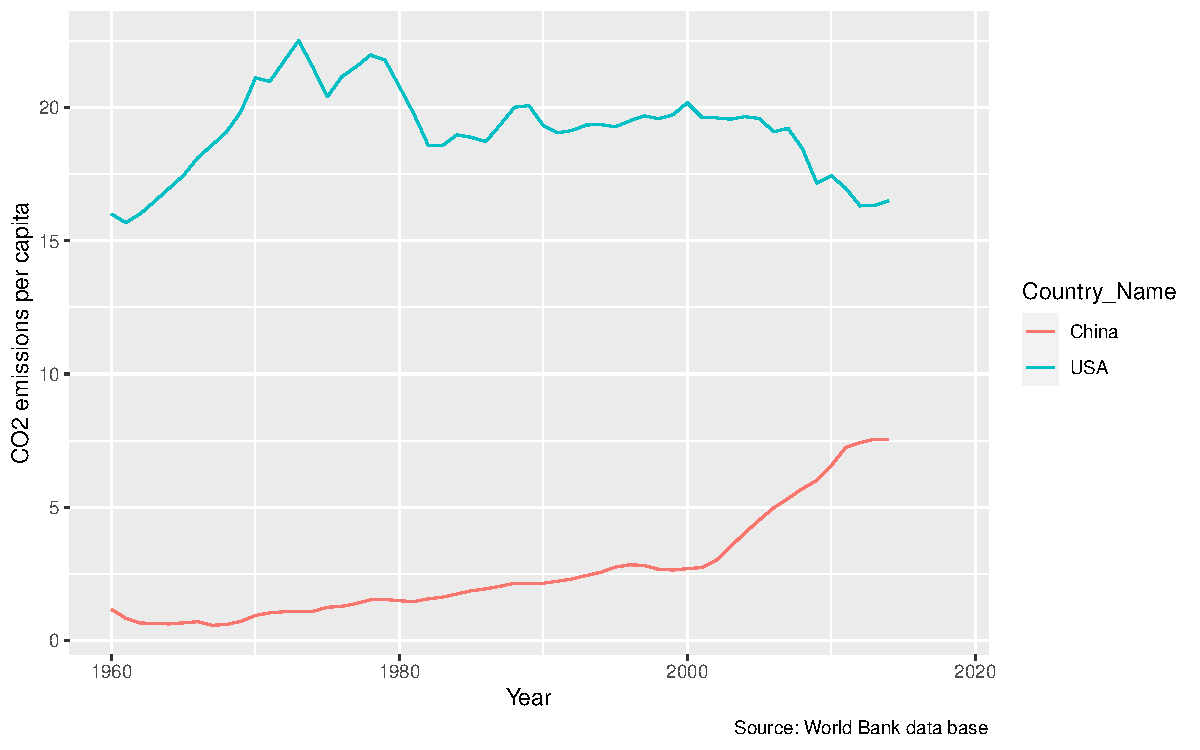
\includegraphics{report_files/figure-latex/fig1-1.pdf}
\caption{\label{fig:fig1}Annual distribution of CO2 emissions in China and USA}
\end{figure}

\section*{Country India and UK}

\hypertarget{research-queations}{%
\subsection{Research Queations}\label{research-queations}}

Q1: We would like to analyze the dependency of CO2 emission on the country's population for India and United Kingdom (UK).

Q2: We would like to analyze the dependency of CO2 emission on the usage of energy from oil in India and United Kingdom (UK).

\hypertarget{question-1-analysis-1}{%
\subsection{Question 1 Analysis}\label{question-1-analysis-1}}

Table \ref{tab:TableIndia} and \ref{tab:TableUK} showing the CO2 emission and population data of India and United Kingdom from 1960-2014, respectively.

\begin{table}[!h]

\caption{\label{tab:TableIndia}CO2 emmission and Urban Population data of India from 1960-2014}
\centering
\begin{tabular}[t]{l|r|r|r}
\hline
Country\_Name & Year & CO2\_emissions\_metric\_tons\_per\_capita & Urban\_population\\
\hline
India & 1960 & 0.2676342 & 80756166\\
\hline
India & 1961 & 0.2837037 & 82882675\\
\hline
India & 1962 & 0.3058510 & 85456482\\
\hline
India & 1963 & 0.3217950 & 88127853\\
\hline
India & 1964 & 0.3081687 & 90901311\\
\hline
India & 1965 & 0.3325272 & 93760316\\
\hline
India & 1966 & 0.3370395 & 96712770\\
\hline
India & 1967 & 0.3309739 & 99765994\\
\hline
India & 1968 & 0.3524575 & 102932967\\
\hline
India & 1969 & 0.3511873 & 106238158\\
\hline
\end{tabular}
\end{table}

\begin{table}[!h]

\caption{\label{tab:TableUK}CO2 emmission and Urban Population data of United Kingdom from 1960-2014}
\centering
\begin{tabular}[t]{l|r|r|r}
\hline
Country\_Name & Year & CO2\_emissions\_metric\_tons\_per\_capita & Urban\_population\\
\hline
UK & 1960 & 11.15076 & 41104656\\
\hline
UK & 1961 & 11.15414 & 41381472\\
\hline
UK & 1962 & 11.14293 & 41661202\\
\hline
UK & 1963 & 11.25485 & 41900114\\
\hline
UK & 1964 & 11.26584 & 42098400\\
\hline
UK & 1965 & 11.45616 & 42294196\\
\hline
UK & 1966 & 11.31896 & 42452048\\
\hline
UK & 1967 & 10.78410 & 42603817\\
\hline
UK & 1968 & 10.99349 & 42733856\\
\hline
UK & 1969 & 11.34267 & 42833742\\
\hline
\end{tabular}
\end{table}

Using Table \ref{tab:TableIndia} and \ref{tab:TableUK} together to analyze the dependency of CO2 emission on the country's population, we create a plot.

\begin{figure}

{\centering 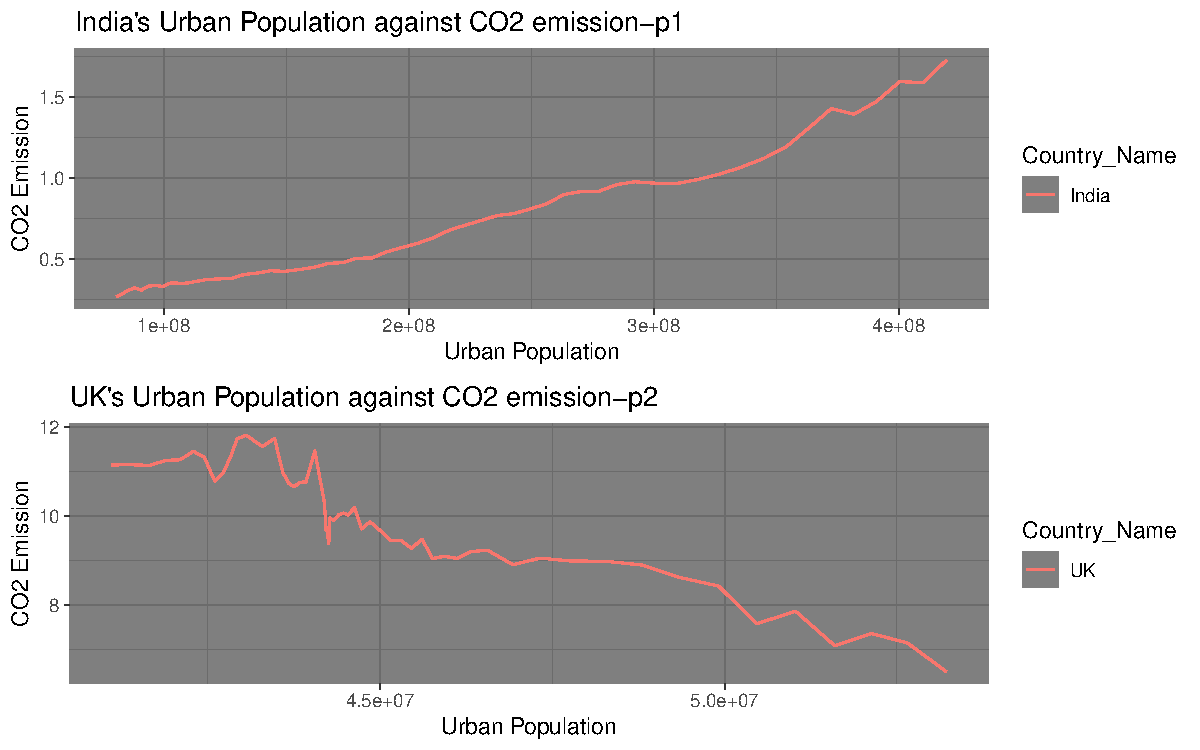
\includegraphics{report_files/figure-latex/plot-1} 

}

\caption{Relationship between CO2 emission and urban population of India and United kingdom}\label{fig:plot}
\end{figure}

The above Figure \ref{fig:plot} shows the relationship between CO2 emission and urban population of India and United Kingdom from the year 1960 to 2014.

According to the above figure \ref{fig:plot}, the plot of India shows an increase in CO2 emission with the increase in urban population which is quite obvious because with the increase in population, CO2 emission should increase and there can be multiple reasons for this like excessive use of vehicles, more industries coming into picture and so on. But in case of United Kingdom, there is an increase in urban population and despite this fact, there is a huge decrease in CO2 emission which is contrary to what we observed in India's case. The possible reason for this might be the deindustrialization in United Kingdom which took place during these years.

\hypertarget{question-2-analysis-1}{%
\subsection{Question 2 Analysis}\label{question-2-analysis-1}}

\begin{table}[!h]

\caption{\label{tab:TableIndia2}CO2 emmission and Energy usage from oil in India from 1971-2014}
\centering
\begin{tabular}[t]{l|r|r|r}
\hline
Country\_Name & Year & CO2\_emissions\_metric\_tons\_per\_capita & Energy\_use\_kg\_of\_oil\_equivalent\_per\_capita\\
\hline
India & 1971 & 0.3625297 & 267.3476\\
\hline
India & 1972 & 0.3748992 & 267.3087\\
\hline
India & 1973 & 0.3771934 & 268.6027\\
\hline
India & 1974 & 0.3810640 & 272.7135\\
\hline
India & 1975 & 0.4047511 & 275.9078\\
\hline
India & 1976 & 0.4136970 & 280.4479\\
\hline
India & 1977 & 0.4277247 & 281.9477\\
\hline
India & 1978 & 0.4241141 & 279.3809\\
\hline
India & 1979 & 0.4346901 & 285.5378\\
\hline
India & 1980 & 0.4492667 & 286.1638\\
\hline
\end{tabular}
\end{table}

\begin{table}[!h]

\caption{\label{tab:TableUK2}CO2 emmission and Energy usage from oil in United Kingdom from 1960-2014}
\centering
\begin{tabular}[t]{l|r|r|r}
\hline
Country\_Name & Year & CO2\_emissions\_metric\_tons\_per\_capita & Energy\_use\_kg\_of\_oil\_equivalent\_per\_capita\\
\hline
UK & 1960 & 11.15076 & 3033.051\\
\hline
UK & 1961 & 11.15414 & 3006.747\\
\hline
UK & 1962 & 11.14293 & 3087.342\\
\hline
UK & 1963 & 11.25485 & 3196.831\\
\hline
UK & 1964 & 11.26584 & 3212.535\\
\hline
UK & 1965 & 11.45616 & 3329.410\\
\hline
UK & 1966 & 11.31896 & 3306.782\\
\hline
UK & 1967 & 10.78410 & 3345.553\\
\hline
UK & 1968 & 10.99349 & 3406.144\\
\hline
UK & 1969 & 11.34267 & 3557.129\\
\hline
\end{tabular}
\end{table}

Table \ref{tab:TableIndia2} and \ref{tab:TableUK2} showing the CO2 emission and Energy usage from oil in India and United Kingdom from 1960-2014, respectively.

Using Table \ref{tab:TableIndia2} and \ref{tab:TableUK2} together to analyze the dependency of CO2 emission on the country's energy usage from oil, we create a plot.

\begin{figure}

{\centering 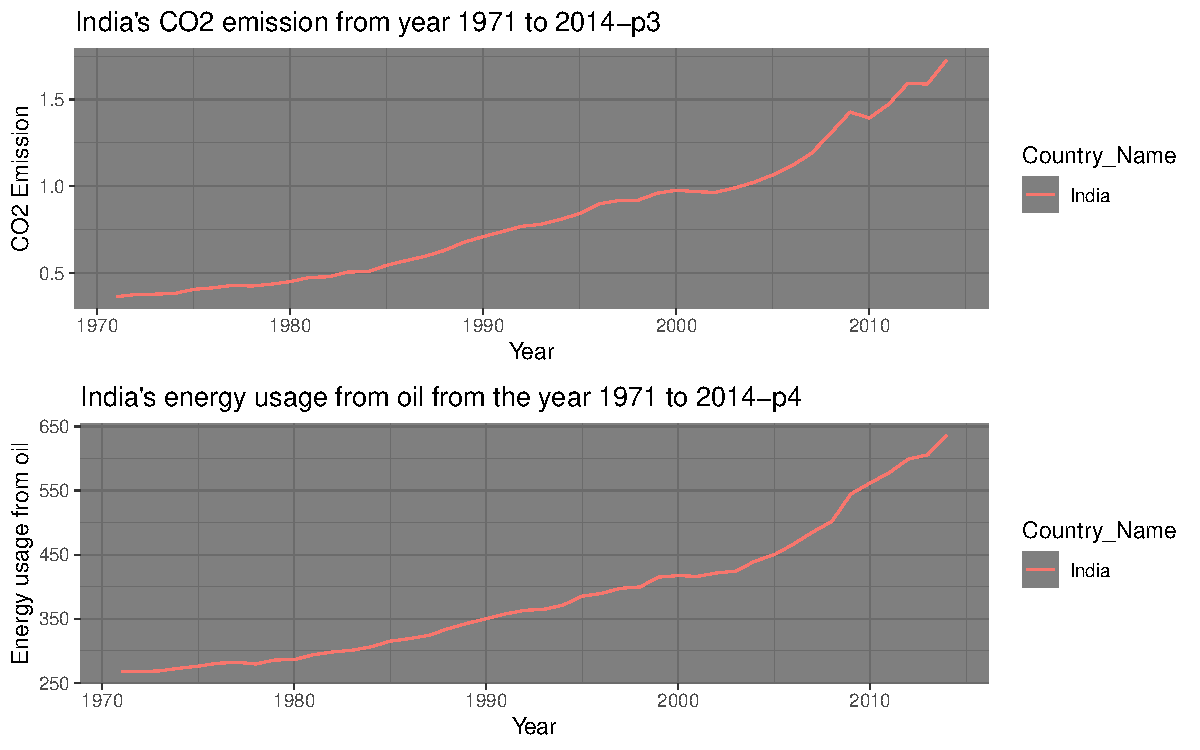
\includegraphics{report_files/figure-latex/plot2-1} 

}

\caption{Relationship between CO2 emission and Energy usage from oil in India}\label{fig:plot2}
\end{figure}

The above Figure \ref{fig:plot2}, shows CO2 emission and energy usage of oil in \textbf{India} from 1971 to 2014. From the above figure \ref{fig:plot2}, we can say that CO2 emission has increased from 1971 to 2014 and the energy usage from oil has also increased from 1971 to 2014. Therefore, it can be inferred that usage of oil for energy production is one of the major factors responsible for increase in CO2 emission in India.

\begin{figure}

{\centering 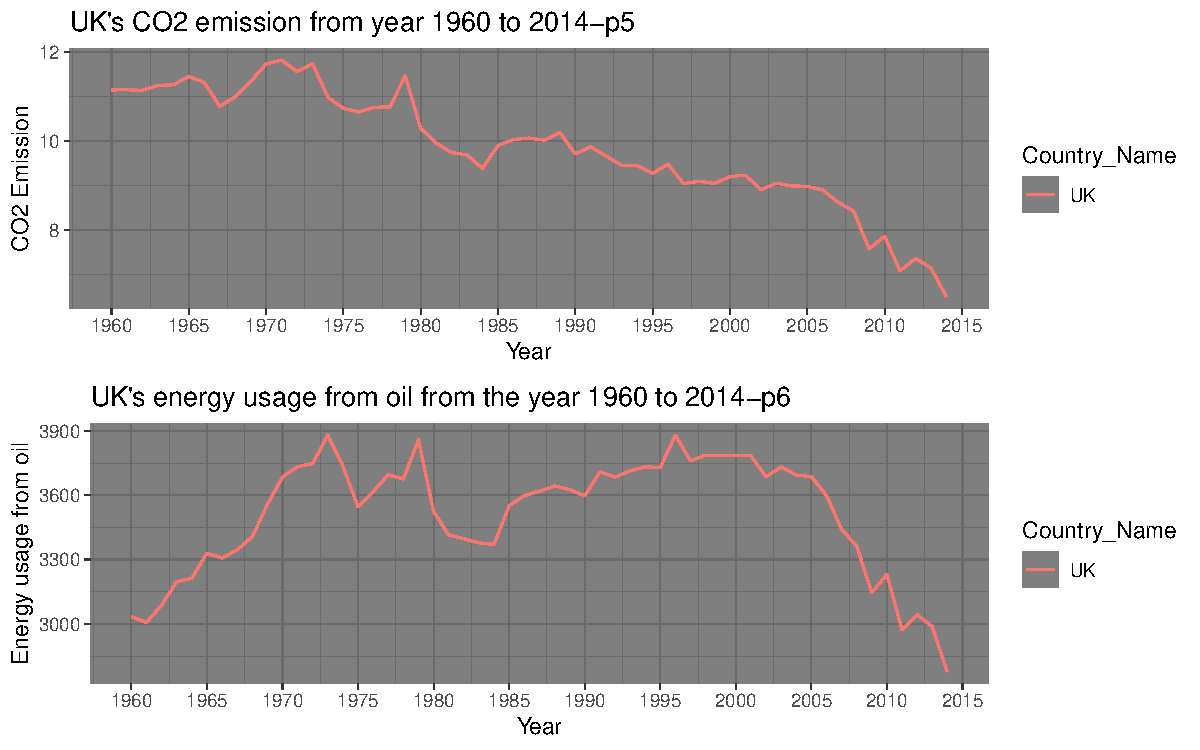
\includegraphics{report_files/figure-latex/plot3-1} 

}

\caption{Relationship between CO2 emission and Energy usage from oil in UK}\label{fig:plot3}
\end{figure}

The above Figure \ref{fig:plot3}, shows CO2 emission and energy usage of oil in \textbf{United Kingdom} from 1960 to 2014. From the above figure \ref{fig:plot3}, we can say that CO2 emission has constantly decreased from 1960 to 2014 while on the other hand, the energy usage from oil has first increased from 1960 to 1980 and then went down a little till 1985. Then from 1985-2000, it has increased again and then after 2000, it has constantly went down. Therefore, it can be inferred that usage of oil for energy production is not related to CO2 emission in UK as it does not follow any specific relation with CO2 emission.

We have also read an Article regarding CO2 emission \textcite{article} which discusses about CO2 emission reduction using various technical measures, using various models and many more. The techniques mentioned in this article might have been used by United Kingdom and that's why we have seen huge CO2 emission reduction in UK despite increase in population.

In order to do the above analysis, the major R packages used by me are \textcite{ggplot2} and \textcite{tidyverse}.

\section*{Country France and Italy}

The article \textcite{ZACHARIADIS2003759} shows a long-term causal relationship between per capita energy consumption and per capita real GDP, and between per capita real GDP and per capita CO2 emissions in squared in Europe.

From the raw data, it can be observed that both France and Italy locate in Europe and belong to high income group. Therefore, in this Section we will compare the CO2 emissions and Energy use between France and Italy, in which people lived in the same region and has a similar income.

\hypertarget{research-questions-1}{%
\subsection{Research Questions}\label{research-questions-1}}

Q1: Which country's people emit more CO2 on average between France and Italy from 1960 to 2014?

Q2: What is the development trend of Energy use in France and Italy from 1960 to 2014?

\hypertarget{question-1-analysis-2}{%
\subsection{Question 1 Analysis}\label{question-1-analysis-2}}

\begin{table}[!h]

\caption{\label{tab:comparation}Comparation of CO2 Emissions between France and Italy}
\centering
\begin{tabular}[t]{lrrr}
\toprule
Country & Ave\_CO2 & Ave\_Energy & Ave\_Population\\
\midrule
France & 6.891838 & 3447.648 & 42958736\\
Italy & 6.366449 & 2355.687 & 37392646\\
\bottomrule
\end{tabular}
\end{table}

The Table \ref{tab:comparation} shows that people in France emit more CO2 than that in Italy, with around 6.89 and 6.37 metric tons per capita respectively.

\clearpage

\hypertarget{question-2-analysis-2}{%
\subsection{Question 2 Analysis}\label{question-2-analysis-2}}

\begin{figure}

{\centering 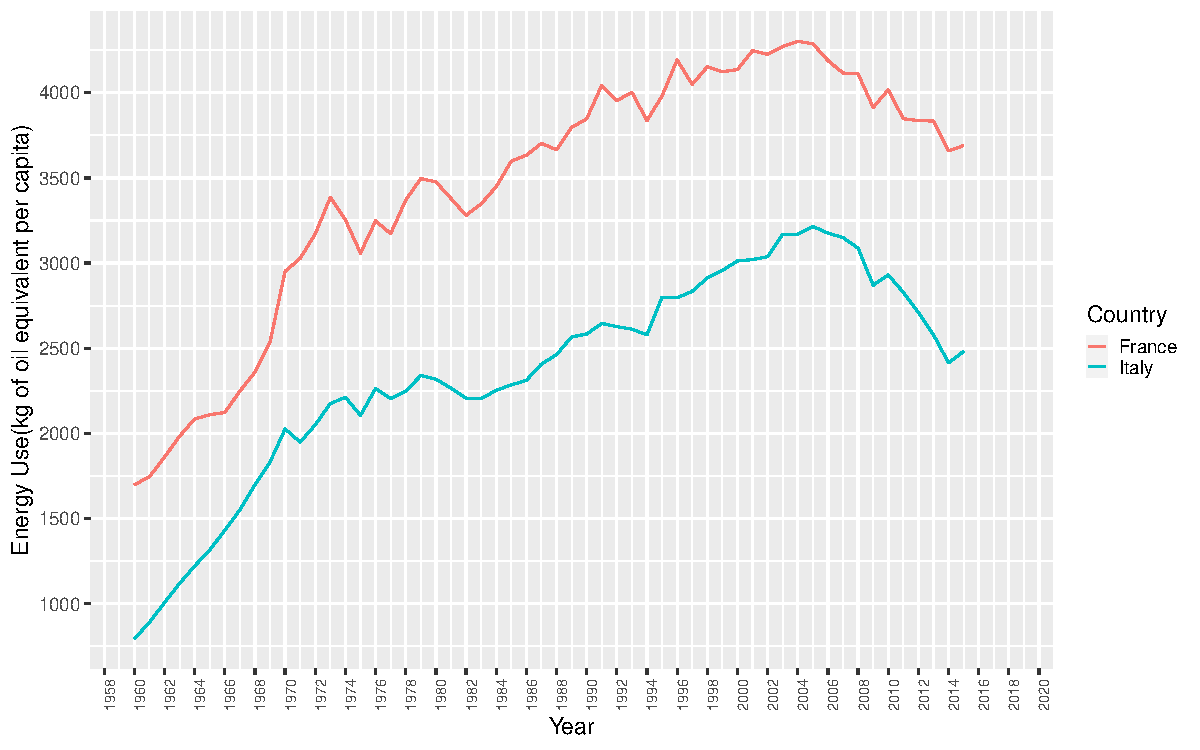
\includegraphics{report_files/figure-latex/trend-1} 

}

\caption{The Trend of Energy Use in France and Italy}\label{fig:trend}
\end{figure}

From the Figure \ref{fig:trend}, we can observe that the trend of energy use (kg of oil equivalent per capita) in France and Italy are similar. They all experienced an increase from 1960 and arrived peak in the year of 2005 at around 4500 and 3250 kg of oil equivalent per capita respectively, and then began to drop until the year of 2015.

\section*{Country Australia and Indonesia}

One of the primary causes of global climate change is Carbon dioxide (CO2) emissions. In the article by \textcite{co2article} , stated that the world needs urgent reductions in emissions to avoid the worst effects of climate change. Hence, in this section, we will look at the trend of CO2 emissions over the year 2004-2014, specifically in Australian and Indonesia, to see which country contributes more to the climate change. Furthermore, does the urban population of each countries has any relation to CO2 emissions.

\clearpage

\hypertarget{research-questions-2}{%
\subsection{Research Questions}\label{research-questions-2}}

Q1: How does CO2 emissions change over the year 2004-2014 in Australia and Indonesia?

Q2: Does higher number of urban population effects the CO2 emissions?

\hypertarget{question-1-analysis-3}{%
\subsection{Question 1 Analysis}\label{question-1-analysis-3}}

From Figure\ref{fig:co2plot}, we can see that Australia has a considerably higher CO2 emission compared to Indonesia. Furthermore, the CO2 emission in Australia has generally decreased over the 10 years, while in Indonesia there was a slight increase with a peak in 2012.

\begin{figure}
\centering
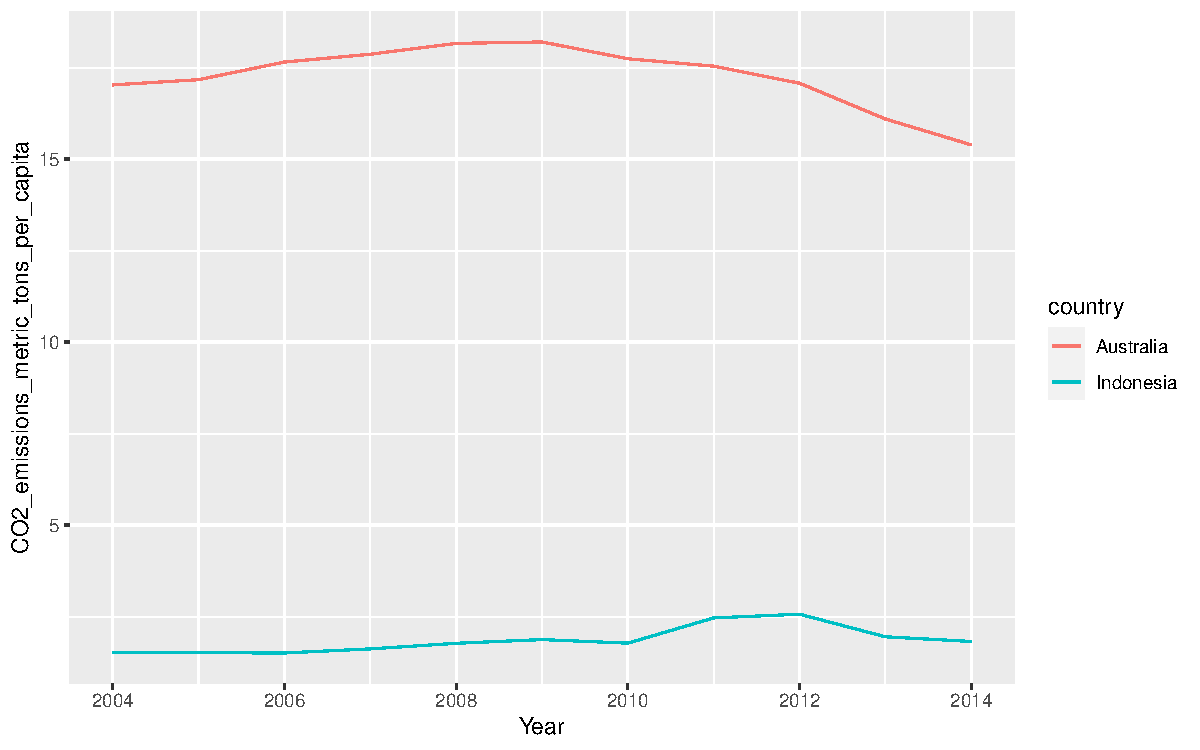
\includegraphics{report_files/figure-latex/co2plot-1.pdf}
\caption{\label{fig:co2plot}The C02 emission of Australia and Indonesia from the year 2004 to 2014}
\end{figure}

\hypertarget{question-2-analysis-3}{%
\subsection{Question 2 Analysis}\label{question-2-analysis-3}}

Table\ref{tab:urbanvsco2} shows that despite having a larger average number of urban population, Indonesia has a much lower CO2 emissions compared to Australia.

\begin{table}[!h]

\caption{\label{tab:urbanvsco2}The average CO2 emissions and urban population of Australia and Indonesia}
\centering
\begin{tabular}[t]{l|r|r}
\hline
Country & Average CO2 emissions (metric tons per capita) & Average Urban Population\\
\hline
Australia & 17.264652 & 18459817\\
\hline
Indonesia & 1.850046 & 117336769\\
\hline
\end{tabular}
\end{table}

Although Australia had a pretty high CO2 emission over 10 years, it has decreased from 2009. On the other hand, Indonesia has a considerably low C02 emission in general, despite of a slight rise over time. Moreover, the analysis suggests that larger urban population might not cause a higher CO2 emission.

\clearpage

\section*{Conclusion}

\begin{itemize}
\item
  From table \ref{tab:Table1}, it can be inferred that in China or USA, CO2 emission or energy consumption is not related to population only, there are other factors as well.
\item
  From the figure \ref{fig:fig1}, it can be inferred that China's per capita CO2 emissions showed an upward trend, while the USA's per capita CO2 emissions stabilized after 1980 and showed a downward trend after 2008.
\item
  From the figure \ref{fig:plot}, it is can be inferred that there might have been an excessive use of vehicles, more industries coming into picture and many more with the increasing population. But in case of United Kingdom, there is a possibility of deindustrialization and use of CO2 emission reducing techniques which reduced CO2 emission in UK despite increasing population.
\item
  From the figure \ref{fig:plot2}, it can be inferred that usage of oil for energy production is one of the major factors responsible for increase in CO2 emission in India.
\item
  From the figure \ref{fig:plot3}, it can be inferred that usage of oil for energy production is not related to CO2 emission in UK as it does not follow any specific relation with CO2 emission.
\item
  From the Table \ref{tab:comparation}, it can be inferred that people in France emit more CO2 than that in Italy, with around 6.89 and 6.37 metric tons per capita respectively. And from the Figure \ref{fig:trend}, we can observe that the trend of energy use (kg of oil equivalent per capita) in France and Italy are similar. They all experienced an increase from 1960 and arrived peak in the year of 2005 at around 4500 and 3250 kg of oil equivalent per capita respectively, and then began to drop until the year of 2015.
\item
  From table \ref{tab:urbanvsco2} it can be inferred that that larger urban population might not cause a higher CO2 emission. There can be other factors which are responsible for CO2 emission like industrialization.
\end{itemize}

\clearpage

\printbibliography

\end{document}
